\section{Twitter-Ebola Dataset}
\label{sec:data_and_model}
\begin{figure*}
\centering
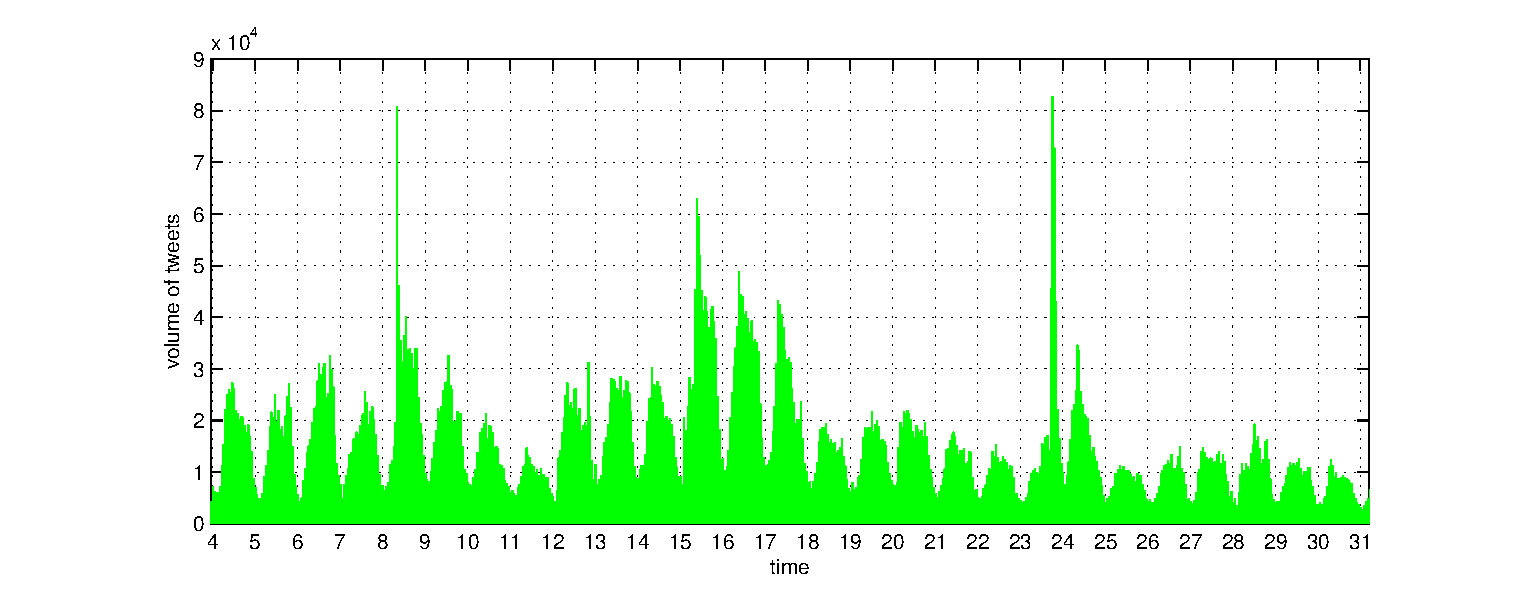
\includegraphics[width=\textwidth]{ICWSM/figures/hashtag_counts_date_time.eps}
\caption{Volume of tweets over time.  Each bin in the \texttt{x-axis} represents 1 hour.  The
\texttt{y-axis} is the volume of tweets during that hour.  The
numbers on the \texttt{x-axis} are the dates during the month of October 2014.  The ticks
on the \texttt{x-axis} coincide with approximately 5 AM of Eastern Standard Time.}
\label{fig:vol_time}
\end{figure*}
The Twitter streaming Application Programming Interface was used to obtain the Twitter messages (tweets) that were published in the
United States in the month of October 2014 with the keywords\footnote{Note that query 
terms were developed with the support of an infectious disease public health specialist.}: 
`\emph{ebola, ebov, ebolavirus, sudan virus, reston virus, bundibugyo virus}'.
From this set, all the non-English tweets were discarded by using the \texttt{user\_lang}
and the \texttt{lang} functionality.
The text of the tweets were preprocessed to exclude any URLs, special characters and hashtags.
A vocabulary count was built from the remaining tweets, and discarded all the word types that appeared
less than $41$ times.  Tweets with only one token were also discarded.  The resulting dataset spans from
October 4 to October 31 totalling 10.5M tweets, and 29000 word types.  This amounts to approximately
375K tweets per day.  After all the data pre-processing such as stopword and infrequent word removal,
the average length of a tweet is approximately 5 words.  
